\documentclass[11pt,landscape,a4paper,fleqn]{article}
\usepackage[utf8]{inputenc}
\usepackage[ngerman]{babel}
\usepackage{tikz}
\usepackage{bbm}
\usetikzlibrary{shapes,positioning,arrows,fit,calc,graphs,graphs.standard}
\usepackage[nosf]{kpfonts}
\usepackage[t1]{sourcesanspro}
%\usepackage[lf]{MyriadPro}
%\usepackage[lf,minionint]{MinionPro}
\usepackage{multicol}
\usepackage{wrapfig}
\usepackage[top=5mm,bottom=5mm,left=5mm,right=5mm]{geometry}
\usepackage[framemethod=tikz]{mdframed}
\usepackage{microtype}
\usepackage{paralist} % for compacter lists
\usepackage{bm}
\usepackage{algorithm}
\usepackage{algpseudocode}
\usepackage{comment}
\usepackage{amsmath}
\usepackage{dsfont}

\makeatletter
\def\BState{\State\hskip-\ALG@thistlm}
\makeatother


\let\bar\overline

\definecolor{myblue}{RGB}{138, 173, 244}
\definecolor{myred}{RGB}{198, 160, 246}
\definecolor{myorange}{RGB}{245, 189, 230}

\pgfdeclarelayer{background}
\pgfsetlayers{background,main}

\everymath\expandafter{\the\everymath \color{myblue}}
%\everydisplay\expandafter{\the\everydisplay \color{myblue}}

\renewcommand{\baselinestretch}{.8}
\pagestyle{empty}

\global\mdfdefinestyle{header}{%
linecolor=gray,linewidth=1pt,%
leftmargin=0mm,rightmargin=0mm,skipbelow=0mm,skipabove=0mm,
}

\makeatletter
\renewcommand{\section}{\@startsection{section}{1}{0mm}%
                                {.2ex}%
                                {.2ex}%x
	                                {\color{myred}\sffamily\small\bfseries}}
\renewcommand{\subsection}{\@startsection{subsection}{1}{0mm}%
                                {.2ex}%
                                {.2ex}%x
                                {\color{myorange}\sffamily\bfseries}}
\renewcommand{\subsubsection}{\@startsection{subsubsection}{1}{0mm}%
	{.2ex}%
	{.2ex}%x
	{\sffamily\bfseries}}


% math helpers
\DeclareMathOperator*{\argmin}{arg\,min}
\DeclareMathOperator*{\argmax}{arg\,max}
\newcommand{\E}{\mathbb{E}}

\makeatother
\setlength{\parindent}{0pt}

\newcommand{\imp}[1]{\boxed{\boldsymbol{#1}}} % Einrahmung und Fett
\newcommand{\w}{\omega}
\newcommand{\ud}{\,\mathrm{d}}% Differential
\newcommand{\norm}[1]{\left\lVert#1\right\rVert}
\newcommand{\X}{\mathcal{X}}
\newcommand{\score}{\text{score}}

% compress equations
%\medmuskip=0mu
%\thinmuskip=0mu
%\thickmuskip=0mu

\begin{document}
\small
\begin{multicols*}{4}
	\section{Basics}
\subsection{Probability}
Bayes rule: $p(y|x) = \frac{p(x|y)p(y)}{p(x)} = \frac{p(x|y)p(y)}{\int p(x|y')p(y')dy'}$\\
$p(y|x)$ \textbf{posterior}, $p(x|y)$ \textbf{likelihood}, $p(y)$ \textbf{prior}, $p(x)$ or $\int p(x|y')p(y')dy'$ \textbf{marginal}
\subsection{Activation Functions}
ReLU(x): $\max(x, 0)$\\
ReLU'(x): $\begin{cases}
		1 & \text{if } x \geq 0 \\
		0 & \text{if } x < 0
	\end{cases}$\\
Leaky ReLU(x): $\begin{cases}
		x     & \text{if } x \geq 0 \\
		0.01x & \text{if } x < 0
	\end{cases}$\\
Leaky ReLU'(x): $\begin{cases}
		1    & \text{if } x \geq 0 \\
		0.01 & \text{if } x < 0
	\end{cases}$\\
Sigmoid: $\sigma(x) = \frac{1}{1 + \exp(-x)}$\\
$\sigma'(x) = \sigma(x)(1-\sigma(x))$\\
Hyperbolic tangent: $\tanh(x) = \frac{\exp(x)-\exp(-x)}{\exp(x)+\exp(-x)}$\\
$\tanh'(x) = 1 - \tanh(x)^2$
	\section{Semirings}
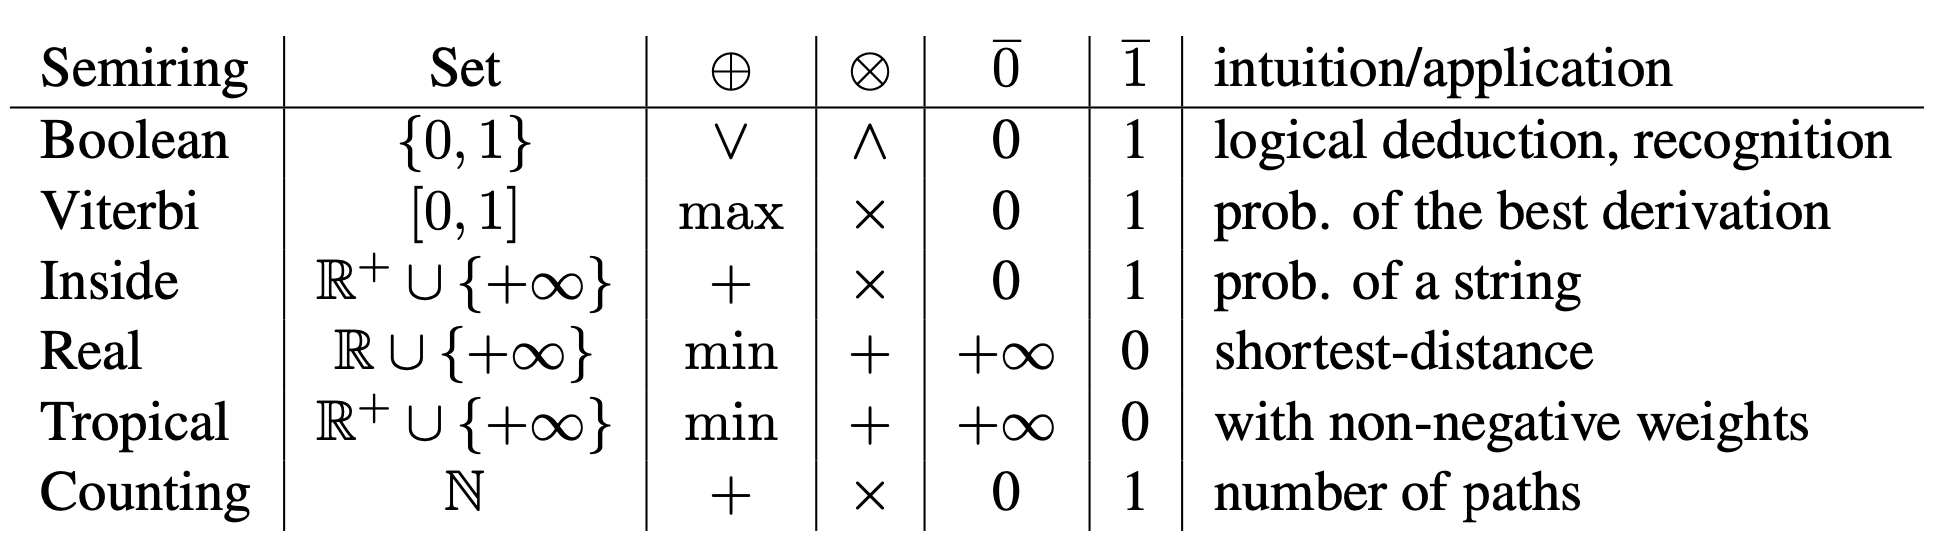
\includegraphics[width=7cm]{semirings.png}
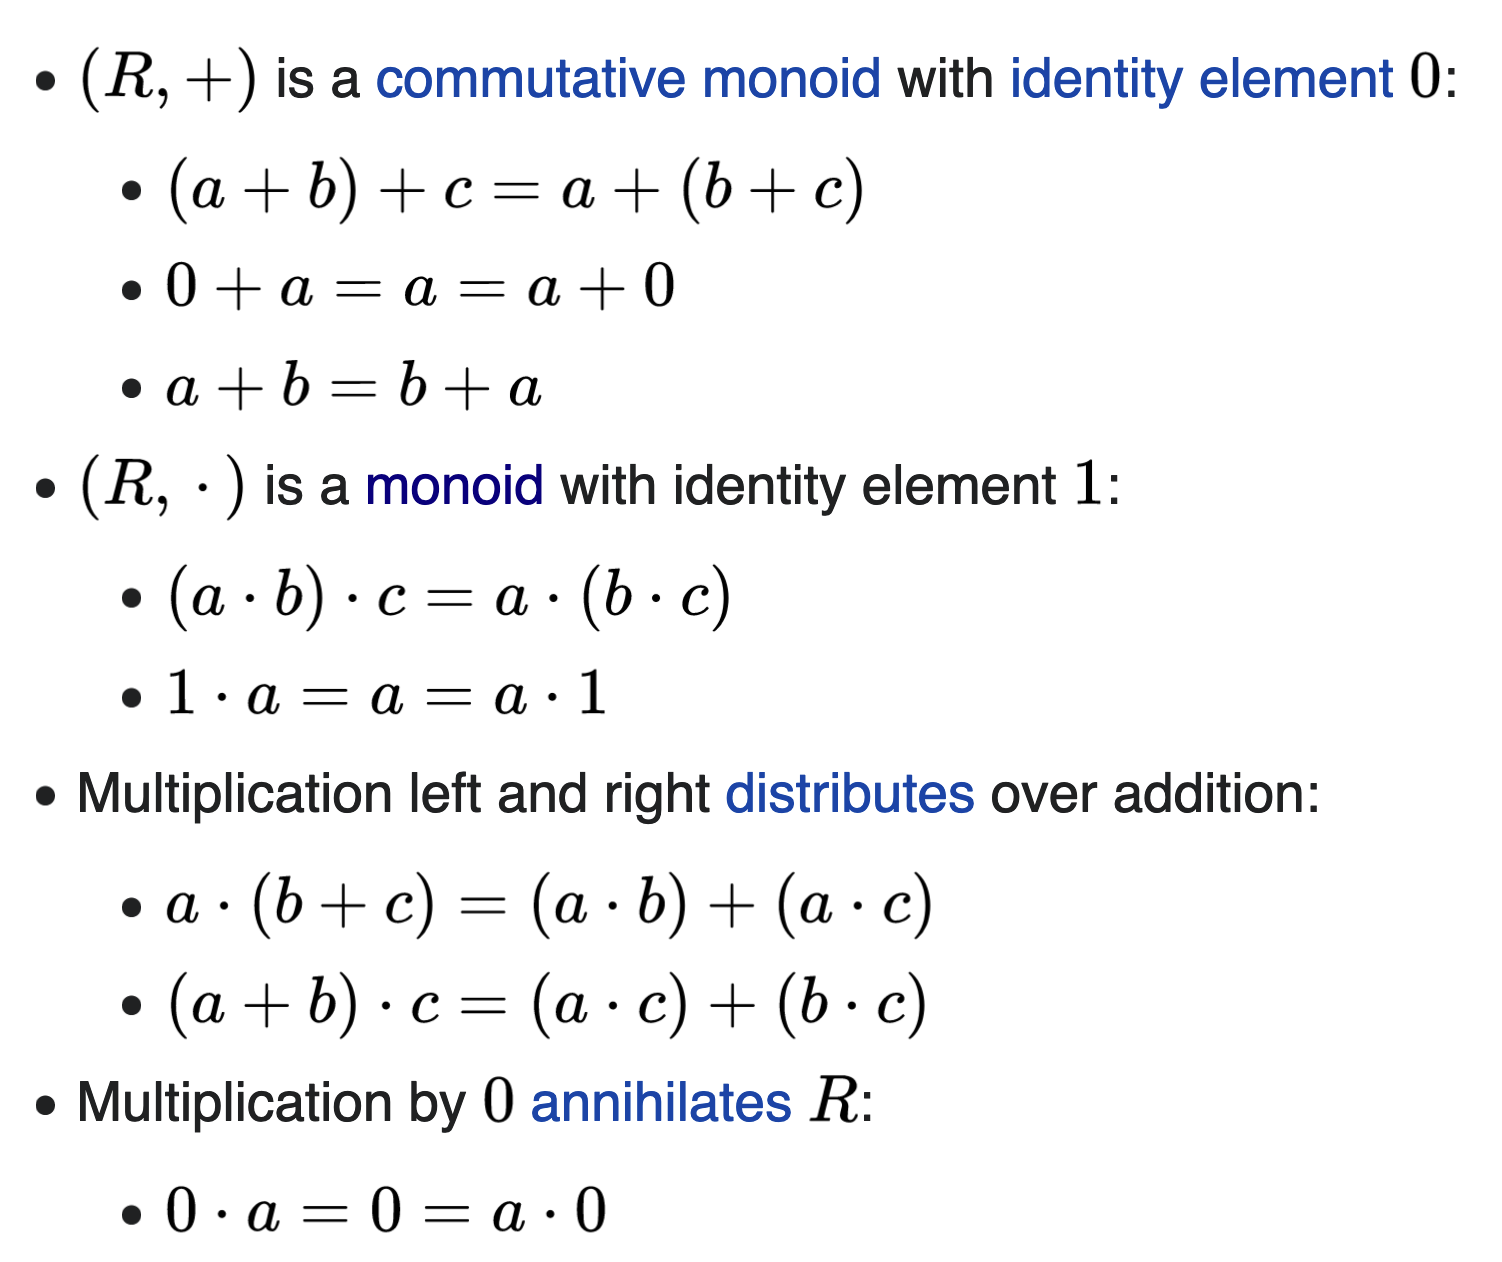
\includegraphics[width=7cm]{semiring_axioms.png}
	\section{Log-Linear Models}
Log-lin. model: $p(y|x, \theta) = \frac{1}{Z(x, \theta)} \exp(\theta f(x, y))$\\
$\log(p(y | x, \theta)) = \theta f(x, y) + \text{const.}$\\
where $f: \mathcal{X} \times \mathcal{Y} \rightarrow \mathbb{R}^K$ is the feature function\\
$Z(\theta) = \sum_{y' \in \mathcal{Y}} \exp(\theta f(x, y'))$ is the partition function.\\
MLE: $\mathcal{L}(\theta) = \sum_{n=1}^{N}\log p(y_n | x_n, \theta)$\\
$\theta_{\text{MLE}} = \argmax_{\theta \in \Theta} \mathcal{L}(\theta)$\\
where $\Theta$ is compact subset of $\mathbb{R}^K$\\
$\bigtriangledown \mathcal{L}(\theta) = \sum_{i=1}^{N} f(x_n, y_n) - \sum_{n=1}^{N} \E_{Y \sim p(\cdot| x_n, \theta)} [f(x_n, Y)]$\\
$\sum_{n \leq N} f(x_n, y_n) = \sum_{n=1}^{N} \E_{Y \sim p(\cdot | x_n, \theta)} [f(x_n, Y)]$
	\section{Viterbi}
$\mathbf{t}^* = \underset{t \in \mathcal{T}^N}{\argmax} \exp(\score(\mathbf{t}, \mathbf{w})) = \underset{t \in \mathcal{T}^N}{\argmax} \prod_{n=1}^{N}\exp \{\score(\langle t_{n-1}, t_n \rangle, w)\}$\\
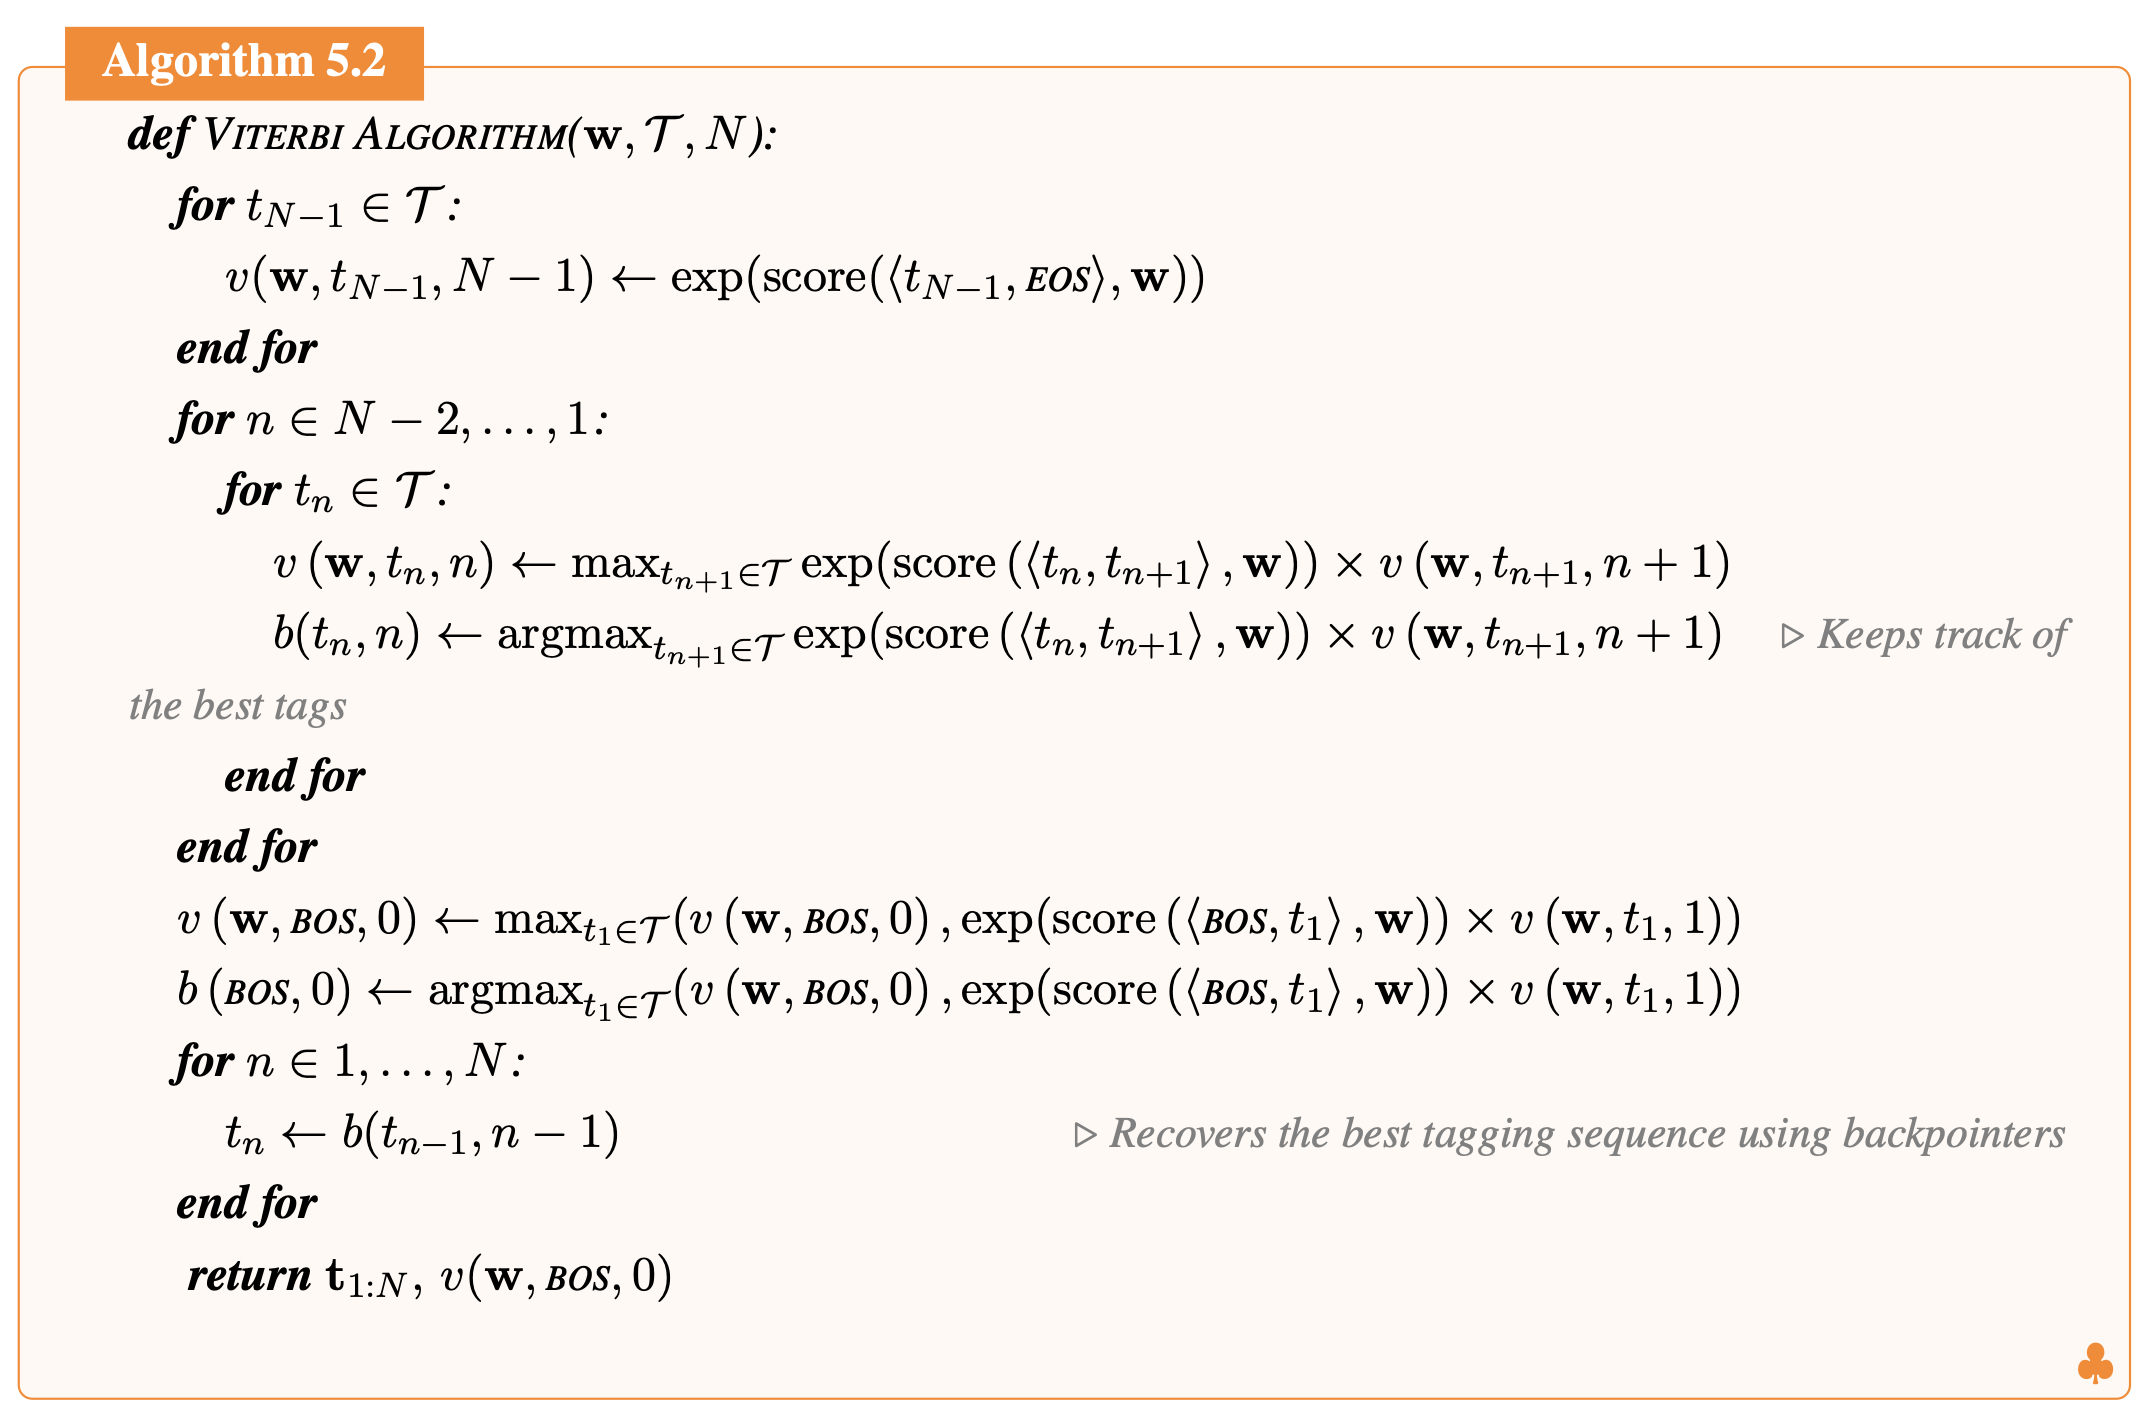
\includegraphics[width=7cm]{viterbi_algo.png}
Runtime: $\mathcal{O}(N|\mathcal{T}|^2)$, $\mathcal{O}(N |\mathcal{T}|^3)$ when considering triplets.
	\section{Grammar}
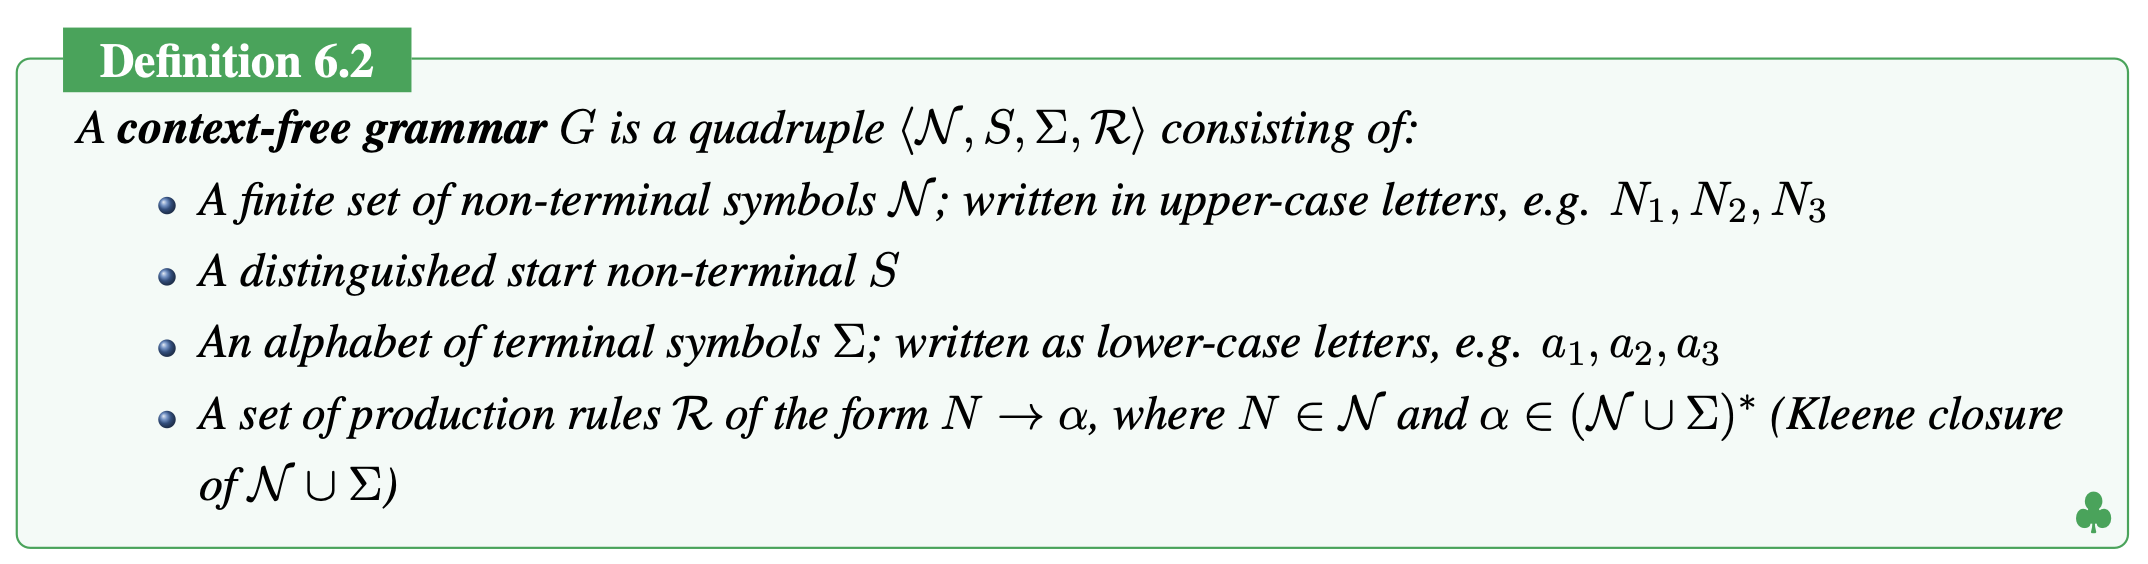
\includegraphics[width=7cm]{cfg_def.png}
\subsection{Chomsky Normal Form}
Grammar is in Chomsky Normal Form (CNF) if RHS of every production rule includes either two non-terminals or a single terminal symbol:
$N_1 \rightarrow N_2 N_3$ or $N \rightarrow a$\\
\subsection{PCFG}
Probabilistic Context Free Grammar (PCFG) $\langle \mathcal{N}, S, \sum, \mathcal{R}, \mathcal{P} \rangle$, where $\mathcal{P}$ are probabilities assigned to each production rule.\\
\subsection{WCFG}
Weighted Context Free Grammar (WCFG) $\langle \mathcal{N}, S, \sum, \mathcal{R}, \mathcal{W} \rangle$, where $\mathcal{W}$ are non-negative weights assigned to each production rule. PCFG is special case of WCFG.
	\section{CKY}
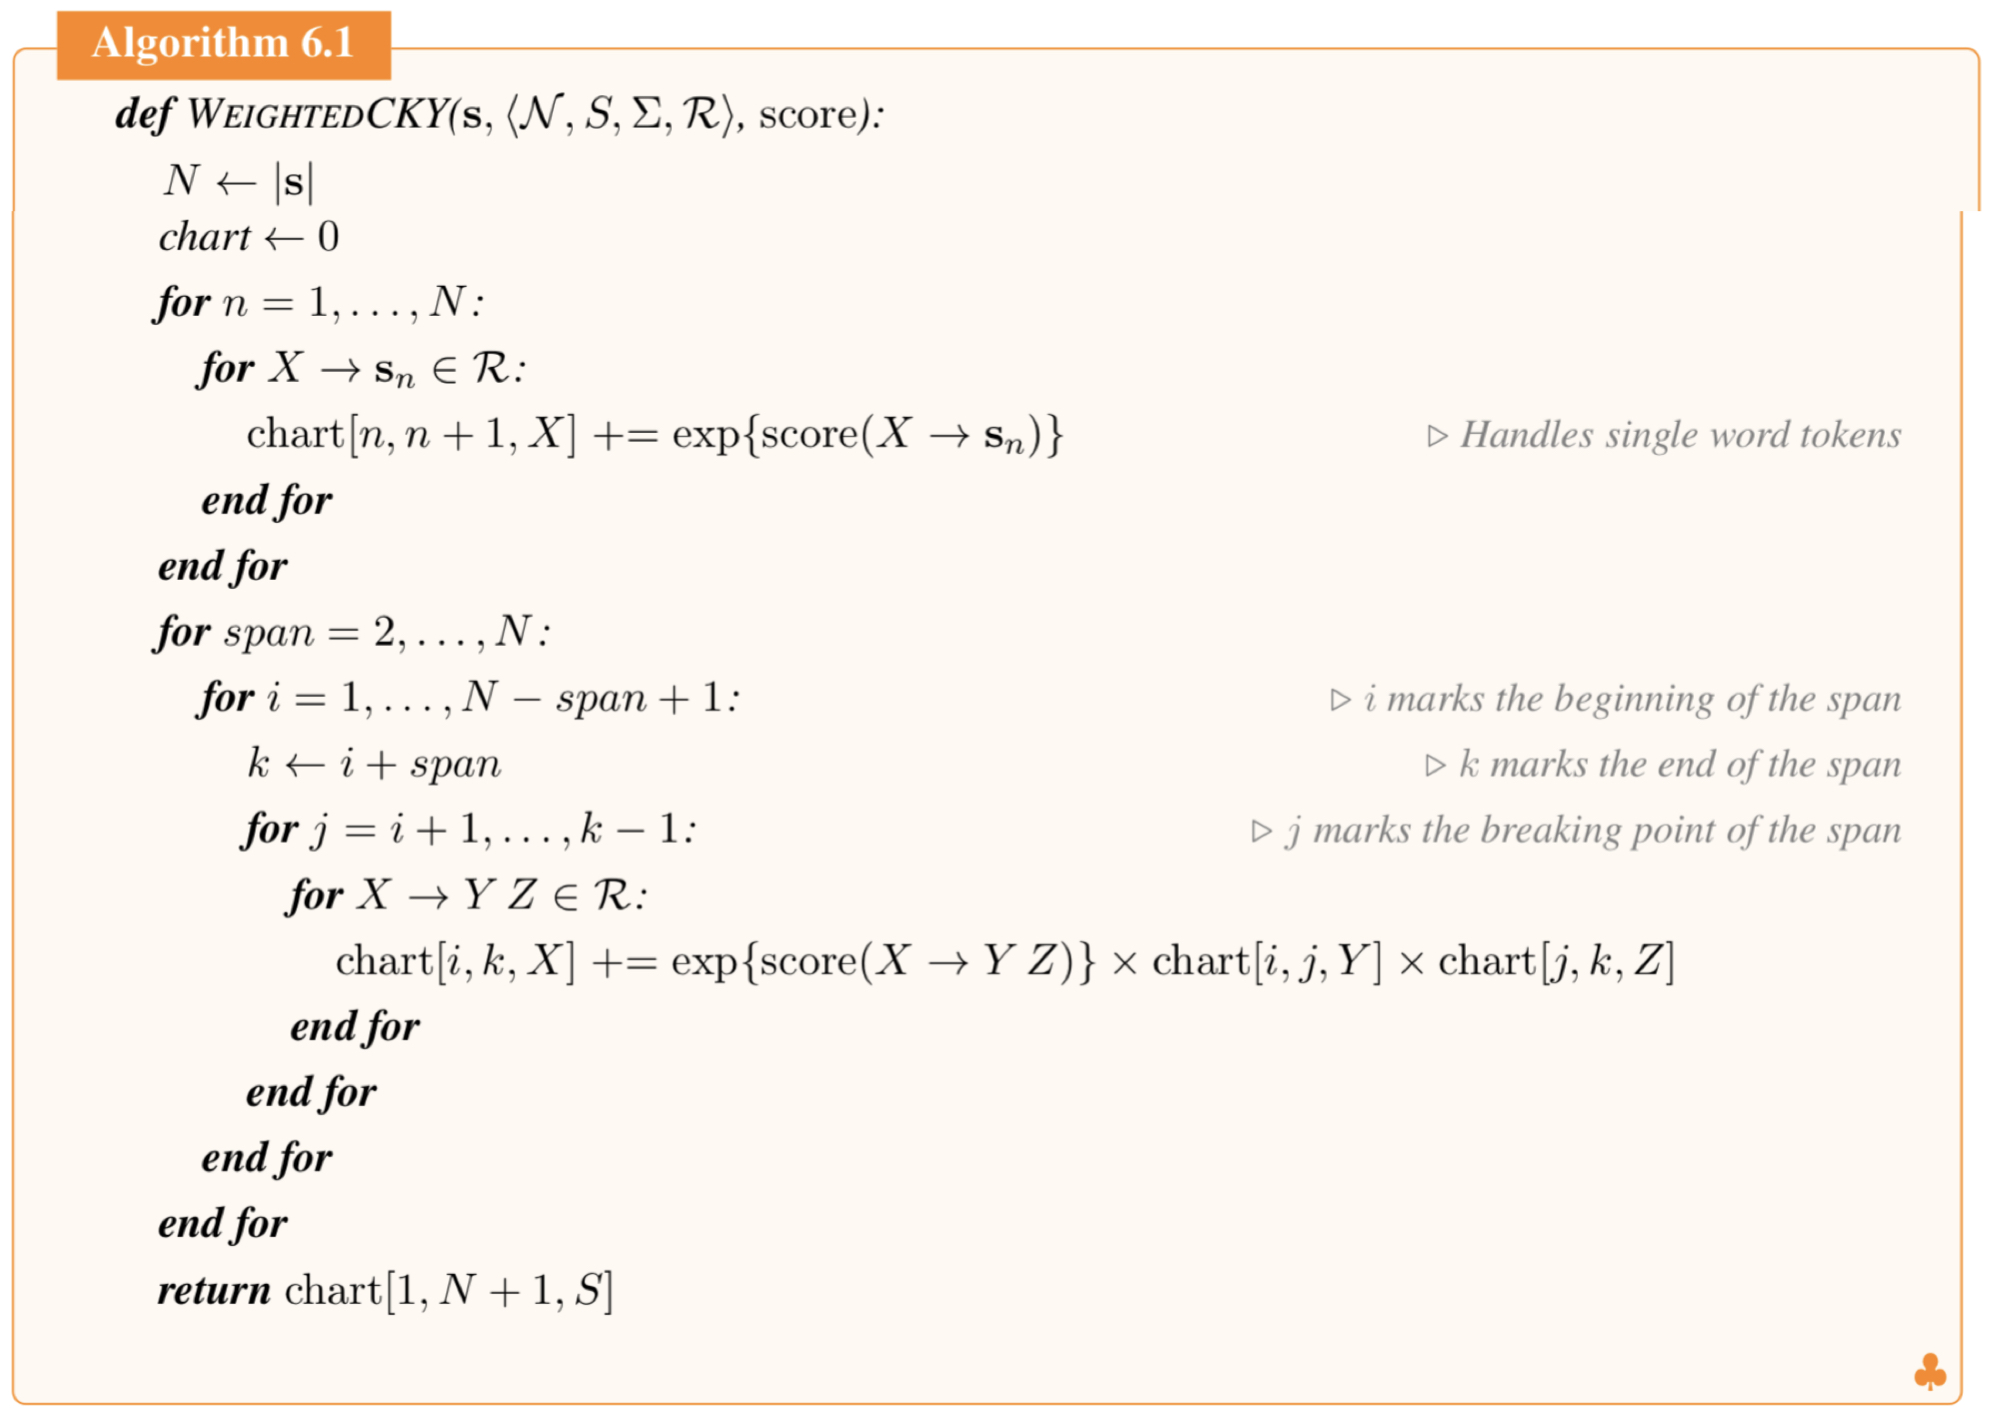
\includegraphics[width=7cm]{cky_algo.jpeg}

	% -*- root: main.tex -*-






	%		\subsection*{Regularization}
	%	The error term $L$ and the regularization $C$ with regularization parameter $\lambda$: $\min \limits_w L(w) + \lambda C(w)$\\
	%	L1-regularization for number of features \\
	%	L2-regularization for the length of $w$

	%	\subsection*{Convex}
	%	$\text{g(x) is convex}$\\
	%	$\Leftrightarrow x_1,x_2 \in \mathbb{R}, \lambda \in [0,1]:$\\
	%	$g(\lambda x_1) + (1-\lambda x_2) \leq \lambda g(x_1) + (1-\lambda) g(x_2)$
	%	$ \Leftrightarrow g''(x) > 0$

	%	\subsection*{Parametric to nonparametric linear regression}
	%	Ansatz: $w=\sum_i \alpha_i x$\\
	%	Parametric: $w^* = \underset{w}{\operatorname{argmin}} \sum_i (*Tx_i-y_i)^2 + \lambda ||w||_2^2$\\
	%	$= \underset{\alpha_{1:n}}{\operatorname{argmin}} \sum \limits_{i=1}^n (\sum \limits_{j=1}^n \alpha_j x_j^T x_i - y_i)^2 + \lambda \sum \limits_i \sum \limits_j \alpha_i \alpha_j (x_i^T x_j)$\\
	%	$= \underset{\alpha_{1:n}}{\operatorname{argmin}} \sum \limits_{i=1}^n (\alpha^T K_i - y_i)^2 + \lambda \alpha^T K \alpha$\\
	%	$= \underset{\alpha}{\operatorname{argmin}} ||\alpha^T K -y||_2^2 + \lambda \alpha^T K \alpha$\\
	%	Closed form: $\alpha^* = (K+\lambda I)^{-1} y$\\
	%	Prediction: $y^*= w^{*^T} x = \sum \limits_{i=1}^n \alpha_i ^* k(x_i,x)$

\end{multicols*}
\end{document}